\documentclass[a4paper,12pt]{article}
\usepackage{polski}
\usepackage[utf8]{inputenc}
\usepackage[OT4]{fontenc}
\usepackage{mathtools}
\usepackage{float}
\usepackage{graphicx}
\usepackage{multirow}
\usepackage{listings}
\usepackage{hyperref}
\usepackage[table,xcdraw]{xcolor}

\begin{document}

%-------------------------------------------------------
%					### TYTUŁOWA ###	

\begin{center}
	\LARGE STRUKTURY DANYCH I ZŁOŻONOŚĆ OBLICZENIOWA\\
	\Large Zadanie projektowe nr 2
	
	\begin{table}[H]
		\centering
		\begin{tabular}{|c|}
			\hline
			\textbf{Temat:}                                                                                                                               \\ \hline
			\begin{tabular}[c]{@{}c@{}}Badanie efektywności algorytmów grafowych.\end{tabular} \\ \hline
			\textbf{Autor:}                                                                                                                               \\ \hline
			Dawid Waligórski                                                                                                                             \\ \hline
			\textbf{Termin zajęć:}                                                                                                                        \\ \hline
			Wtorek, godz. 15.15, TP                                                                                                                      \\ \hline
		\end{tabular}
	\end{table}
	
\end{center}

\newpage

\tableofcontents

\newpage

%-------------------------------------------------------
%	CEL ZADANIA PROJEKTOWEGO
\section{Założenia projektowe:}

\subsection{Cele projektu:}
Celem projektu była implementacja algorytmów grafowych wraz z niezbędnymi do ich działania strukturami danych w języku C++. Kluczowym było również dokonanie pomiaru czasów wykonywania się wspomnianych algorytmów na grafach o różnych reprezentacjach, rozmiarach (liczba wierzchołków) oraz gęstościach (liczba krawędzi). Badanymi algorytmami były:
\begin{itemize}
	\item Algorytm Prima (problem wyznaczenia MST)
	\item Algorytm Kruskala (problem wyznaczenia MST)
	\item Algorytm Dijkstry (problem wyszukiwania najkrótszych ścieżek)
	\item Algorytm Bellmana-Forda (problem wyszukiwania najkrótszych ścieżek)
\end{itemize}
\vspace{5mm}

\noindent
Tworzona aplikacja z konsolowym interfejsem użytkownika, poza możliwością przeprowadzenia eksperymentów miała oferować również opcję sprawdzenia poprawności zaimplementowanych algorytmów za pomocą dedykowanych menu.\\

\subsection{Grafy:}
Założono, że wierzchołki grafu będą identyfikowane przez kolejne, nieujemne liczby całkowite (typ \it unsigned int\rm). Do przechowywania wartości krawędzi wybrano znakowany, 4-bajtowy typ całkowity (\it int\rm). W zależności od wybranego problemu mogły być one skierowane (najkrótsza ścieżka) lub nieskierowane (MST).\\

\noindent
Badane algorytmy otrzymać miały swoje odpowiedniki dla dwóch różnych sposobów reprezentacji grafu. Pierwszy z nich zakładał użycie macierzy sąsiedztwa. Drugi korzystać miał ze zbioru połączonych list sąsiadów. W wypadku macierzy sąsiedztwa, zamiast tradycyjnej, binarnej informacji o istnieniu krawędzi między wierzchołkami, miała ona zawierać informację o wadze krawędzi. Brak połączenia w tej strukturze był oznaczany za pomocą specjalnej, zarezerwowanej wartości NO\_CONNECTION (wartość minimalna typu \it int\rm).\\

\noindent
Dodatkowo możliwym miało być wczytanie grafu z pliku (np. tekstowego). Pierwsza linia w takim pliku definiować miała liczbę wierzchołków, krawędzi, a także wierzchołki początkowy i końcowy (wykorzystywane przy niektórych algorytmach). W kolejnych liniach znajdować się miały dane na temat kolejnych krawędzi grafu w konwencji: wierzchołek początkowy, wierzchołek końcowy, waga.

%-------------------------------------------------------
%	METODA POMIAROWA
\section{Metoda pomiarowa:}

\subsection{Środowisko pomiarowe:}
Pomiary przeprowadzano na komputerze stacjonarnym z zainstalowanym systemem Windows 10 (wersja 64-bitowa). Częstotliwość taktowania zegara procesora wynosiła 3,60GHz. Ilość pamięci operacyjnej wynosiła 16GB. W trakcie pomiarów na maszynie działały jedynie niezbędne do funkcjonowania systemu operacyjnego procesy. Aplikacja mierząca działała w domyślnym trybie przydziału zasobów komputera. Była ona skompilowana za pomocą narzędzia \it g++ \rm na poziomie optymalizacji O3. 

\subsection{Pomiary wykonywane w programie:}

\subsubsection{Narzędzie pomiarowe:}
W pomiarach czasu wykorzystano specjalną klasę \it Timer\rm. Instancja wspomnianej klasy działała na zasadzie stopera, mierząc czas pomiędzy wywołaniami swoich metod \it start() \rm oraz \it stop()\rm. Precyzja prowadzonego nią pomiaru była rzędu 0,1 mikrosekundy ($10^{-7}s$). Przykład użycia \it Timer \rm został zamieszczony na rysunku \ref{timer-przyklad}.
\begin{figure}[H]
	\centering
	\caption{\centering Przykład użycia klasy \it Timer \rm do pomiaru czasu wykonania algorytmu Bellmana-Forda.}
	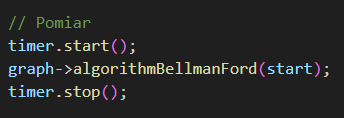
\includegraphics[width=7cm]{fig2.png}
	\label{fig.timer-przyklad}
\end{figure}

\subsubsection{Przebieg pomiaru:}
Pomiary czasu wykonywania algorytmów zostały wkomponowane jako jedne z opcji możliwych do wyboru z poziomu aplikacji projektowej (rys. \ref{fig.opcja-badanie}). W wypadku wybrania takiej opcji aplikacja dawała użytkownikowi opcję wyboru algorytmu, który miał zostać przebadany. Następnie wykonywany był właściwy pomiar, dzielący się na 40 faz. Każda faza wyróżniała się inną kombinacją parametrów używanego w pomiarach grafu. Owe parametry oraz ich dopuszczalne wartości zamieszczono w tabeli \ref{tab-parametry}. W trakcie jednej fazy wykonywano łącznie 100 prób. Dla każdej z osobna generowano nową, losową instancję grafu (odpowiedniego dla danego algorytmu). Później za pomocą klasy \it Timer \rm dokonywano pomiaru czasu wykonywania wybranego algorytmu. W końcu dane o próbie były zapisywane w specjalnej strukturze, która po zakończeniu się danej fazy była zapisywana do pliku \it *.csv \rm w formie jednego z jego z rekordów. Pola takiego rekordu została zamieszczona w tabeli \ref{tab.wynik-pomairu}.
\begin{figure}[H]
	\centering
	\caption{\centering Menu główne, zawierające opcję przeprowadzenia pomiarów.}
	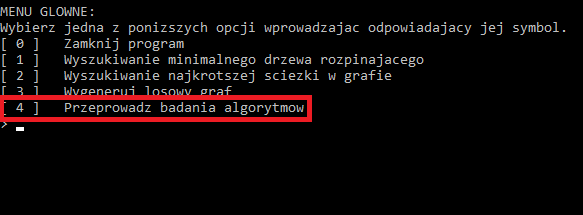
\includegraphics[width=12cm]{fig1.png}
	\label{fig.opcja-badanie}
\end{figure}

\begin{table}[H]
	\centering
	\caption{\centering Tabela zawierające parametry grafów używanych w poszczególnych fazach badania wraz z ich dopuszczalnymi wartościami.}
	\label{tab-parametry}
	\begin{tabular}{|l|c|c|c|}
		\hline
		\textbf{Parametr:}  & Reprezentacja                                                             & Rozmiar                                                             & Gęstość                                                                                                              \\ \hline
		\textbf{Opis:}     & \begin{tabular}[c]{@{}c@{}}Sposób \\ reprezentacji \\ grafu.\end{tabular} & \begin{tabular}[c]{@{}c@{}}Liczba \\ wierzchołków.\end{tabular}     & \begin{tabular}[c]{@{}c@{}}Stosunek liczby krawędzi \\ grafu do jego \\ maksymalnej \\ liczby krawędzi.\end{tabular} \\ \hline
		\textbf{Wartości:} & \begin{tabular}[c]{@{}c@{}}listowa\\ macierzowa\end{tabular}              & \begin{tabular}[c]{@{}c@{}}100\\ 200\\ 300\\ 400\\ 500\end{tabular} & \begin{tabular}[c]{@{}c@{}}25\%\\ 50\%\\ 75\%\\ 99\%\end{tabular}                                                    \\ \hline
	\end{tabular}
\end{table}

\begin{table}[H]
	\centering
	\label{tab.wynik-pomairu}
	\caption{\centering Tabela zawierająca strukturę rekordu pliku \it *.csv\rm, zawierającego wyniki pomiarów.}
	\begin{tabular}{|l|l|}
		\hline
		\textbf{Algorytm}      & Inicjał odpowiadający badanemu algorytmowi. \\ \hline
		\textbf{Reprezentacja} & Typ reprezentacji przebadanego grafu.       \\ \hline
		\textbf{Rozmiar}       & Rozmiar przebadanego grafu.                 \\ \hline
		\textbf{Gęstość}       & Gęstość przebadanego grafu.                 \\ \hline
		\textbf{Czas}          & Zmierzony czas.                             \\ \hline
	\end{tabular}
\end{table}

\subsubsection{Generowanie grafu:}
Za generowanie losowych instancji grafów, używanych w badaniach odpowiedzialna była klasa \it GraphGenerator\rm. Była ona paremetryzowana wartościami takimi jak:
\begin{itemize}
	\item Typ reprezentacji grafu
	\item Liczba wierzchołków
	\item Informacja o skierowaniu krawędzi
	\item Gęstość grafu
	\item Informacja o dopuszczalności wystąpienia ujemnych wag krawędzi
\end{itemize}
\vspace{5mm}

\noindent
Tak duża gama parametrów pozwoliła na generowanie grafów dobrze przystosowanych do każdego z zaimplementowanych algorytmów (np. zabraniając generowania się ujemnych krawędzi w wypadku algorytmu Dijkstry).\\

\noindent
Najważniejszym i najbardziej wymagającym zadaniem powierzonym omawianej klasie było generowanie losowego zbioru krawędzi dla tworzonego grafu. Było ono wykonywane w dwóch etapach. W pierwszym generowane, a następnie umieszczane w tablicy były wszystkie, możliwe dla danego typu grafu (skierowany/nieskierowany) krawędzie. Drugi etap polegał na wybraniu z uzyskanej kolekcji krawędzi losowego podzbioru o wielkości podyktowanej przez parametr gęstości grafu. Odbywało się to poprzez kolejne losowania indeksu z wygenerowanej w etapie pierwszym tablicy, stale pomniejszanej o już wybrane krawędzie. Spójność generowanego grafu była zapewniana jeszcze przed wspomnianym losowaniem, poprzez wylosowanie $|V|-1$ krawędzi, tworzących jedno z drzew rozpinających grafu (wygenerowanie grafu o mniejszej ilości krawędzi jest niemożliwe).

\subsection{Przetworzenie wyników w arkuszu kalkulacyjnym:}
Z pojedynczego pliku wynikowego \it*.csv\rm, uzyskanego na skutek zakończenia się jednej fazy pomiarów otrzymywano 100 rekordów, z których wyliczano parametr $t$. Jest to średni czas wykonywania operacji mierzonej w danej fazie. Wspomniany parametr wraz z odpowiadającą mu wielkością grafu ($V$) oraz gęstością grafu ($d$) umieszczono w tabelach opisujących zależności $t(V)$ dla danych gęstości oraz reprezentacji grafu ($R$). Wszystkie wartości w nich zawarte zaokrąglono do dwóch cyfr znaczących.\\

\noindent	
Dla wspomnianych tabel wyliczono ponadto dodatkowy parametr $c$ wraz z jego względnym odchyleniem standardowym ($\sigma$), który służył do sprawdzenia spójności uzyskanych wyników z zależnościami teoretycznymi. Wynika on bezpośrednio z teoretycznych złożoności (wzory \ref{eq.c-1} oraz \ref{eq.c-2}), które powinny przyjąć implementowane algorytmy. W wypadku w implementacji w pełni zgodnej z teorią wartość $c$ powinna pozostać relatywnie stała dla każdego wpisu w tabeli dla danej gęstości i reprezentacji.

\begin{equation}
	\label{eq.c-1}
	t = c \cdot E \cdot \log_{2}V \implies c = \frac{t}{E \cdot \log_{2}V} = const
\end{equation}

\begin{equation}
	\label{eq.c-2}
	t = c \cdot E \cdot V \implies c = \frac{t}{E \cdot V} = const
\end{equation}
\vspace{1mm}

\noindent
Wyniki naniesiono również na cztery wykresy, pozwalające na porównanie złożoności algorytmów tyczących się tego samego typu problemu dla grafu o danej reprezentacji. Na każdym z nich wykreślono linie obrazujące zależności $t(V)$ dla grafów o różnych gęstościach. Stworzonymi wykresami były:
\begin{itemize}
	\item Porównanie algorytmów wyznaczania MST dla reprezentacji macierzowej (rys. \ref{fig.wykres-macierz-mst})
	\item Porównanie algorytmów wyznaczania MST dla reprezentacji listowej (rys. \ref{fig.wykres-lista-mst})
	\item Porównanie algorytmów wyszukiwania najkrótszej ścieżki dla reprezentacji macierzowej (rys. \ref{fig.wykres-macierz-shortpath})
	\item Porównanie algorytmów wyszukiwania najkrótszej ścieżki dla reprezentacji listowej (rys. \ref{fig.wykres-lista-shortpath})
\end{itemize} 

%-------------------------------------------------------
%	WYZNACZANIE MINIMALNEGO DRZEWA SPINAJĄCEGO
\section{Wyznaczanie MST:}

\subsection{Algorytm Prima:}

\subsubsection{Opis teoretyczny:}
Algorytm Prima jest zachłannym algorytmem pozwalającym na wyznaczenie minimalnego drzewa rozpinającego grafu. Zakłada się przy tym, że graf, na którym wykonywany jest algorytm jest grafem spójnym, o krawędziach nieskierowanych.\\

\noindent
Pierwszym krokiem algorytmu Prima jest wybranie dowolnego wierzchołka startowego. Następnie, iteracyjnie dodawane są do MST kolejne krawędzie, łączące z drzewem wierzchołki do niego nienależące, zaczynając od krawędzi o najmniejszej wadze. Proces ten trwa do momentu, gdy wszystkie wierzchołki staną się częścią minimalnego drzewa rozpinającego.\\

\noindent
Książkowa implementacja algorytmu zakłada użycie kolejki priorytetowej (kopca minimalnego), przechowującej krawędzie, która pozwoli na łatwy dostęp do krawędzi o minimalnej wadze. Taki dostęp będzie mieć wówczas złożoność jednostkową $O(1)$. Dodawanie krawędzi do wspomnianej kolejki będzie miało złożoność $O(\log E)$. W ramach optymalizacji zamiast krawędzi można przechowywać w kopcu pary w postaci: indeks wierzchołka, indeks krawędzi o minimalnej wadze od niego prowadzącej. Wówczas kolejka będzie krótsza, a złożoność dodawania do niej elementu wyniesie $O(\log V)$. W najgorszym wypadku, gdy musimy rozważyć wszystkie krawędzie grafu, aby wyznaczyć MST, wspomniane wcześniej operacje należy powtórzyć dla każdej krawędzi, a więc $E$ razy. W efekcie daje to łączną złożoność algorytmu równą $O(E \cdot \log V)$.

\subsubsection{Zastosowana implementacja:}
Przy implementacji algorytmu Dijkstry wykorzystano kolejkę priorytetową. Była ona de facto zmodyfikowanym kopcem, stworzonym na potrzeby poprzedniego zadania projektowego. Zamiast liczb całkowitych ze znakiem przechowywał on strukturę o polach: indeks wierzchołka, sąsiad z przypisanej krawędzi, waga przypisanej krawędzi. W celu zoptymalizowania operacji dodawania i usuwania elementów pozbyto się przymusu każdorazowej relokacji kopca, występującego przy tychże działaniach. Dokonano tego poprzez zwirtualizowanie tychże operacji. Rzeczywisty rozmiar tablicy, na której bazował kopiec pozostawał stały. Zmniejszany bądź zwiększany był jedynie jej obszar uznawany w danym momencie za właściwy kopiec.\\

\noindent
De facto zdecydowano się także na przechowywanie nadmiarowych elementów w kopcu. W teoretycznej implementacji, zakładającej przechowywanie wierzchołków w kopcu, istnieje wymóg zmieniania przypisywanej im wagi w wypadku znalezienia takiej krawędzi łączącej go z drzewem, której waga byłaby mniejsza od tej aktualnie przypisanej do wierzchołka. Taka operacja wymagałaby jego uprzedniego odnalezienia w kopcu. Tak operacja miałaby złożoność $O(V)$ i znacznie spowolniłaby działanie algorytmu. W związku z tym zrezygnowano z jej użycia.

\subsection{Algorytm Kruskala:}

\subsubsection{Opis teoretyczny:}
Algorytm Kruskala jest algorytmem grafowym, pozwalającym na wyznaczenie minimalnego drzewa rozpinającego grafu. Zakłada się przy tym, że graf, na którym wykonywany jest algorytm jest grafem spójnym, o krawędziach nieskierowanych.\\

\noindent
Pierwszym krokiem algorytmu Kruskala jest posortowanie krawędzi grafu niemalejąco. Następnie do MST dodawane jest pierwsze $|V|-1$ krawędzi z posortowanego zbioru, które nie spowodują powstania cyklu w budowanym drzewie. Ów proces zaczyna się od krawędzi o minimalnej wadze. Kończy się w momencie, gdy wszystkie wierzchołki zostaną zawarte w wyznaczanym MST. \\

\noindent
Teoretyczna implementacja nie narzuca żadnego konkretnego typu sortowania. Zakłada się, że wykorzystany algorytm będzie mieć w najgorszym wypadku złożoność $O(E \cdot \log E)$. Jako, że w grafach skierowanych maksymalna liczba krawędzi jest mniejsza od wartości $V^2$, a więc prawdziwa jest równość $\log E < 2\log V$, to złożoność części sortującej szacuje się na de facto $O (E \log V)$. Drugą fazę algorytmu, dodającą krawędzie do drzewa, przy jednoczesnym upewnieniu się, że nie tworzą one cyklu, realizuje najczęściej się za pomocą specjalnej struktury zbiorów rozłącznych. Jej zastosowanie sprawia, że złożoność czasowa tej części wynosi $O(E \cdot \alpha(E,V))$, gdzie $\alpha$ jest funkcją rosnącą znacznie wolniej od funkcji klasy $n \log n$. Z tego powodu łączna złożoność algorytmu jest dyktowana przez jego partię sortującą i wynosi $O (E \cdot \log V)$.

\subsubsection{Zastosowana implementacja:}
W wypadku algorytmu Kruskala zdecydowano się na użycie algorytmu sortującego typu quick-sort. Miał on złożoność czasową równą $O(E \log E)$. W drugiej fazie, zgodnie z teorią, wykorzystano strukturę zbiorów rozłącznych, pozwalającą na efektywne działanie algorytmu.\\

\noindent
Wprowadzono także dodatkową poprawkę, która pozwalała w niektórych przypadkach na przedwczesne zakończenie się algorytmu. W wypadku, gdy odnotowano wybranie ze zbioru krawędzi grafu $V-1$ elementów, rezygnowano z rozważania kolejnych krawędzi. W takiej sytuacji wiadomym było, że MST zostało już w pełni wyznaczone.

\subsection{Wyniki pomiarów:}

\begin{table}[H]
	\centering
	\caption{\centering Wyniki pomiarów dla algorytmu Prima wykonywanego na grafie w reprezentacji macierzowej o gęstości 25\%.}
	\begin{tabular}{|c|c|c|c|c|c|}
		\hline
		\rowcolor[HTML]{C0C0C0} 
		$R$                       & $d$                    & $V$ & $t$    & $c$                & $\sigma$               \\ \hline
		&                        & 100 & 0,14ms & 1,7$\cdot 10^{-5}$ &                        \\ \cline{3-5}
		&                        & 200 & 0,50ms & 1,3$\cdot 10^{-5}$ &                        \\ \cline{3-5}
		&                        & 300 & 1,1ms  & 1,2$\cdot 10^{-5}$ &                        \\ \cline{3-5}
		&                        & 400 & 2,0ms  & 1,1$\cdot 10^{-5}$ &                        \\ \cline{3-5}
		\multirow{-5}{*}{macierz} & \multirow{-5}{*}{25\%} & 500 & 3,0ms  & 1,1$\cdot 10^{-5}$ & \multirow{-5}{*}{18\%} \\ \hline
	\end{tabular}
\end{table}

\begin{table}[H]
	\centering
	\caption{\centering Wyniki pomiarów dla algorytmu Prima wykonywanego na grafie w reprezentacji macierzowej o gęstości 50\%.}
	\begin{tabular}{|c|c|c|c|c|c|}
		\hline
		\rowcolor[HTML]{C0C0C0} 
		$R$                       & $d$                    & $V$ & $t$    & $c$                 & $\sigma$               \\ \hline
		&                        & 100 & 0,20ms & 1,2$\cdot 10^{-5}$  &                        \\ \cline{3-5}
		&                        & 200 & 0,76ms & 1,0$\cdot 10^{-5}$  &                        \\ \cline{3-5}
		&                        & 300 & 1,7ms  & 0,91$\cdot 10^{-5}$ &                        \\ \cline{3-5}
		&                        & 400 & 2,9ms  & 0,85$\cdot 10^{-5}$ &                        \\ \cline{3-5}
		\multirow{-5}{*}{macierz} & \multirow{-5}{*}{50\%} & 500 & 4,8ms  & 0,85$\cdot 10^{-5}$ & \multirow{-5}{*}{17\%} \\ \hline
	\end{tabular}
\end{table}

\begin{table}[H]
	\centering
	\caption{\centering Wyniki pomiarów dla algorytmu Prima wykonywanego na grafie w reprezentacji macierzowej o gęstości 75\%.}
	\begin{tabular}{|c|c|c|l|c|c|}
		\hline
		\rowcolor[HTML]{C0C0C0} 
		$R$                       & $d$                    & $V$ & \multicolumn{1}{c|}{\cellcolor[HTML]{C0C0C0}$t$} & $c$                & $\sigma$               \\ \hline
		&                        & 100 & 0,23ms                                           & 9,4$\cdot 10^{-6}$ &                        \\ \cline{3-5}
		&                        & 200 & 0,87ms                                           & 7,6$\cdot 10^{-6}$ &                        \\ \cline{3-5}
		&                        & 300 & 1,9ms                                            & 6,9$\cdot 10^{-6}$ &                        \\ \cline{3-5}
		&                        & 400 & 3,4ms                                            & 6,5$\cdot 10^{-6}$ &                        \\ \cline{3-5}
		\multirow{-5}{*}{macierz} & \multirow{-5}{*}{75\%} & 500 & 5,4ms                                            & 6,5$\cdot 10^{-6}$ & \multirow{-5}{*}{17\%} \\ \hline
	\end{tabular}
\end{table}

\begin{table}[H]
	\centering
	\caption{\centering Wyniki pomiarów dla algorytmu Prima wykonywanego na grafie w reprezentacji macierzowej o gęstości 99\%.}
	\begin{tabular}{|c|c|c|c|c|c|}
		\hline
		\rowcolor[HTML]{C0C0C0} 
		$R$                       & $d$                    & $V$ & \multicolumn{1}{c|}{\cellcolor[HTML]{C0C0C0}$t$} & $c$                & $\sigma$               \\ \hline
		&                        & 100 & 0,25ms                                           & 7,7$\cdot 10^{-6}$ &                        \\ \cline{3-5}
		&                        & 200 & 0,94ms                                           & 6,3$\cdot 10^{-6}$ &                        \\ \cline{3-5}
		&                        & 300 & 2,1ms                                            & 5,7$\cdot 10^{-6}$ &                        \\ \cline{3-5}
		&                        & 400 & 3,7ms                                            & 5,4$\cdot 10^{-6}$ &                        \\ \cline{3-5}
		\multirow{-5}{*}{macierz} & \multirow{-5}{*}{99\%} & 500 & 5,9ms                                            & 5,4$\cdot 10^{-6}$ & \multirow{-5}{*}{16\%} \\ \hline
	\end{tabular}
\end{table}

\begin{table}[H]
	\centering
	\caption{\centering Wyniki pomiarów dla algorytmu Kruskala wykonywanego na grafie w reprezentacji macierzowej o gęstości 25\%.}
	\begin{tabular}{|c|c|c|c|c|c|}
		\hline
		\rowcolor[HTML]{C0C0C0} 
		$R$                       & $d$                    & $V$ & \multicolumn{1}{c|}{\cellcolor[HTML]{C0C0C0}$t$} & $c$                & $\sigma$                \\ \hline
		&                        & 100 & 0,14ms                                           & 1,7$\cdot 10^{-5}$ &                         \\ \cline{3-5}
		&                        & 200 & 0,55ms                                           & 1,4$\cdot 10^{-5}$ &                         \\ \cline{3-5}
		&                        & 300 & 1,3ms                                            & 1,5$\cdot 10^{-5}$ &                         \\ \cline{3-5}
		&                        & 400 & 2,6ms                                            & 1,5$\cdot 10^{-5}$ &                         \\ \cline{3-5}
		\multirow{-5}{*}{macierz} & \multirow{-5}{*}{25\%} & 500 & 4,3ms                                            & 1,5$\cdot 10^{-5}$ & \multirow{-5}{*}{7,9\%} \\ \hline
	\end{tabular}
\end{table}

\begin{table}[H]
	\centering
	\caption{\centering Wyniki pomiarów dla algorytmu Kruskala wykonywanego na grafie w reprezentacji macierzowej o gęstości 50\%.}
	\begin{tabular}{|c|c|c|c|c|c|}
		\hline
		\rowcolor[HTML]{C0C0C0} 
		$R$                       & $d$                    & $V$ & $t$    & $c$                & $\sigma$               \\ \hline
		&                        & 100 & 0,24ms & 1,5$\cdot 10^{-5}$ &                        \\ \cline{3-5}
		&                        & 200 & 0,99ms & 1,3$\cdot 10^{-5}$ &                        \\ \cline{3-5}
		&                        & 300 & 2,5ms  & 1,4$\cdot 10^{-5}$ &                        \\ \cline{3-5}
		&                        & 400 & 5,1ms  & 1,5$\cdot 10^{-5}$ &                        \\ \cline{3-5}
		\multirow{-5}{*}{macierz} & \multirow{-5}{*}{50\%} & 500 & 9,6ms  & 1,7$\cdot 10^{-5}$ & \multirow{-5}{*}{11\%} \\ \hline
	\end{tabular}
\end{table}

\begin{table}[H]
	\centering
	\caption{\centering Wyniki pomiarów dla algorytmu Kruskala wykonywanego na grafie w reprezentacji macierzowej o gęstości 75\%.}
	\begin{tabular}{|c|c|c|c|c|c|}
		\hline
		\rowcolor[HTML]{C0C0C0} 
		$R$                       & $d$                    & $V$ & \multicolumn{1}{c|}{\cellcolor[HTML]{C0C0C0}$t$} & $c$                & $\sigma$               \\ \hline
		&                        & 100 & 0,32ms                                           & 1,3$\cdot 10^{-5}$ &                        \\ \cline{3-5}
		&                        & 200 & 1,5ms                                            & 1,3$\cdot 10^{-5}$ &                        \\ \cline{3-5}
		&                        & 300 & 3,8ms                                            & 1,4$\cdot 10^{-5}$ &                        \\ \cline{3-5}
		&                        & 400 & 8,3ms                                            & 1,6$\cdot 10^{-5}$ &                        \\ \cline{3-5}
		\multirow{-5}{*}{macierz} & \multirow{-5}{*}{75\%} & 500 & 17ms                                             & 2,0$\cdot 10^{-5}$ & \multirow{-5}{*}{19\%} \\ \hline
	\end{tabular}
\end{table}

\begin{table}[H]
	\centering
	\caption{\centering Wyniki pomiarów dla algorytmu Kruskala wykonywanego na grafie w reprezentacji macierzowej o gęstości 99\%.}
	\begin{tabular}{|c|c|c|c|c|c|}
		\hline
		\rowcolor[HTML]{C0C0C0} 
		$R$                       & $d$                    & $V$ & $t$    & $c$                & $\sigma$               \\ \hline
		&                        & 100 & 0,41ms & 1,2$\cdot 10^{-5}$ &                        \\ \cline{3-5}
		&                        & 200 & 1,9ms  & 1,3$\cdot 10^{-5}$ &                        \\ \cline{3-5}
		&                        & 300 & 5,3ms  & 1,5$\cdot 10^{-5}$ &                        \\ \cline{3-5}
		&                        & 400 & 12ms   & 1,8$\cdot 10^{-5}$ &                        \\ \cline{3-5}
		\multirow{-5}{*}{macierz} & \multirow{-5}{*}{99\%} & 500 & 25ms   & 2,2$\cdot 10^{-5}$ & \multirow{-5}{*}{26\%} \\ \hline
	\end{tabular}
\end{table}

\begin{table}[H]
	\centering
	\caption{\centering Wyniki pomiarów dla algorytmu Prima wykonywanego na grafie w reprezentacji listowej o gęstości 25\%.}
	\begin{tabular}{|c|c|c|c|c|c|}
		\hline
		\rowcolor[HTML]{C0C0C0} 
		$R$                     & $d$                    & $V$ & $t$    & $c$                & $\sigma$               \\ \hline
		&                        & 100 & 0,16ms & 1,9$\cdot 10^{-5}$ &                        \\ \cline{3-5}
		&                        & 200 & 0,95ms & 2,5$\cdot 10^{-5}$ &                        \\ \cline{3-5}
		&                        & 300 & 3,5ms  & 3,8$\cdot 10^{-5}$ &                        \\ \cline{3-5}
		&                        & 400 & 10ms   & 6,0$\cdot 10^{-5}$ &                        \\ \cline{3-5}
		\multirow{-5}{*}{lista} & \multirow{-5}{*}{25\%} & 500 & 23ms   & 8,3$\cdot 10^{-5}$ & \multirow{-5}{*}{59\%} \\ \hline
	\end{tabular}
\end{table}

\begin{table}[H]
	\centering
	\caption{\centering Wyniki pomiarów dla algorytmu Prima wykonywanego na grafie w reprezentacji listowej o gęstości 50\%.}
	\begin{tabular}{|c|c|c|c|c|c|}
		\hline
		\rowcolor[HTML]{C0C0C0} 
		$R$                     & $d$                    & $V$ & $t$    & $c$                 & $\sigma$               \\ \hline
		&                        & 100 & 0,41ms & 2,5$\cdot 10^{-5}$  &                        \\ \cline{3-5}
		&                        & 200 & 3,9ms  & 5,2$\cdot 10^{-5}$  &                        \\ \cline{3-5}
		&                        & 300 & 18ms   & 9,5$\cdot 10^{-5}$  &                        \\ \cline{3-5}
		&                        & 400 & 47ms   & 0,14$\cdot 10^{-5}$ &                        \\ \cline{3-5}
		\multirow{-5}{*}{lista} & \multirow{-5}{*}{50\%} & 500 & 99ms   & 0,18$\cdot 10^{-5}$ & \multirow{-5}{*}{64\%} \\ \hline
	\end{tabular}
\end{table}

\begin{table}[H]
	\centering
	\caption{\centering Wyniki pomiarów dla algorytmu Prima wykonywanego na grafie w reprezentacji listowej o gęstości 75\%.}
	\begin{tabular}{|c|c|c|c|c|c|}
		\hline
		\rowcolor[HTML]{C0C0C0} 
		$R$                     & $d$                    & $V$ & $t$    & $c$                 & $\sigma$               \\ \hline
		&                        & 100 & 0,83ms & 3,4$\cdot 10^{-5}$  &                        \\ \cline{3-5}
		&                        & 200 & 11ms   & 9,9$\cdot 10^{-5}$  &                        \\ \cline{3-5}
		&                        & 300 & 46ms   & 0,17$\cdot 10^{-5}$ &                        \\ \cline{3-5}
		&                        & 400 & 120ms  & 0,23$\cdot 10^{-5}$ &                        \\ \cline{3-5}
		\multirow{-5}{*}{lista} & \multirow{-5}{*}{75\%} & 500 & 250ms  & 0,29$\cdot 10^{-5}$ & \multirow{-5}{*}{62\%} \\ \hline
	\end{tabular}
\end{table}

\begin{table}[H]
	\centering
	\caption{\centering Wyniki pomiarów dla algorytmu Prima wykonywanego na grafie w reprezentacji listowej o gęstości 99\%.}
	\begin{tabular}{|c|c|c|c|c|c|}
		\hline
		\rowcolor[HTML]{C0C0C0} 
		$R$                     & $d$                    & $V$ & \multicolumn{1}{c|}{\cellcolor[HTML]{C0C0C0}$t$} & $c$                 & $\sigma$               \\ \hline
		&                        & 100 & 1,6ms                                            & 4,9$\cdot 10^{-5}$  &                        \\ \cline{3-5}
		&                        & 200 & 22ms                                             & 0,15$\cdot 10^{-5}$ &                        \\ \cline{3-5}
		&                        & 300 & 86ms                                             & 0,24$\cdot 10^{-5}$ &                        \\ \cline{3-5}
		&                        & 400 & 220ms                                            & 0,33$\cdot 10^{-5}$ &                        \\ \cline{3-5}
		\multirow{-5}{*}{lista} & \multirow{-5}{*}{99\%} & 500 & 470ms                                            & 0,43$\cdot 10^{-5}$ & \multirow{-5}{*}{62\%} \\ \hline
	\end{tabular}
\end{table}

\begin{table}[H]
	\centering
	\caption{\centering Wyniki pomiarów dla algorytmu Kruskala wykonywanego na grafie w reprezentacji listowej o gęstości 25\%.}
	\begin{tabular}{|c|c|c|c|c|c|}
		\hline
		\rowcolor[HTML]{C0C0C0} 
		$R$                     & $d$                    & $V$ & $t$    & $c$                & $\sigma$               \\ \hline
		&                        & 100 & 0,18ms & 2,2$\cdot 10^{-5}$ &                        \\ \cline{3-5}
		&                        & 200 & 1,1ms  & 2,8$\cdot 10^{-5}$ &                        \\ \cline{3-5}
		&                        & 300 & 3,8ms  & 4,1$\cdot 10^{-5}$ &                        \\ \cline{3-5}
		&                        & 400 & 11ms   & 6,3$\cdot 10^{-5}$ &                        \\ \cline{3-5}
		\multirow{-5}{*}{lista} & \multirow{-5}{*}{25\%} & 500 & 24ms   & 8,7$\cdot 10^{-5}$ & \multirow{-5}{*}{55\%} \\ \hline
	\end{tabular}
\end{table}

\begin{table}[H]
	\centering
	\caption{\centering Wyniki pomiarów dla algorytmu Kruskala wykonywanego na grafie w reprezentacji listowej o gęstości 50\%.}
	\begin{tabular}{|c|c|c|c|c|c|}
		\hline
		\rowcolor[HTML]{C0C0C0} 
		$R$                     & $d$                    & $V$ & $t$    & $c$                 & $\sigma$               \\ \hline
		&                        & 100 & 0,47ms & 5,8$\cdot 10^{-5}$  &                        \\ \cline{3-5}
		&                        & 200 & 4,3ms  & 0,11$\cdot 10^{-5}$ &                        \\ \cline{3-5}
		&                        & 300 & 19ms   & 0,21$\cdot 10^{-5}$ &                        \\ \cline{3-5}
		&                        & 400 & 51ms   & 0,30$\cdot 10^{-5}$ &                        \\ \cline{3-5}
		\multirow{-5}{*}{lista} & \multirow{-5}{*}{50\%} & 500 & 110ms  & 0,39$\cdot 10^{-5}$ & \multirow{-5}{*}{63\%} \\ \hline
	\end{tabular}
\end{table}

\begin{table}[H]
	\centering
	\caption{\centering Wyniki pomiarów dla algorytmu Kruskala wykonywanego na grafie w reprezentacji listowej o gęstości 75\%.}
	\begin{tabular}{|c|c|c|c|c|c|}
		\hline
		\rowcolor[HTML]{C0C0C0} 
		$R$                     & $d$                    & $V$ & $t$    & $c$                 & $\sigma$               \\ \hline
		&                        & 100 & 0,96ms & 3,9$\cdot 10^{-5}$  &                        \\ \cline{3-5}
		&                        & 200 & 12ms   & 0,11$\cdot 10^{-5}$ &                        \\ \cline{3-5}
		&                        & 300 & 50ms   & 0,18$\cdot 10^{-5}$ &                        \\ \cline{3-5}
		&                        & 400 & 130ms  & 0,25$\cdot 10^{-5}$ &                        \\ \cline{3-5}
		\multirow{-5}{*}{lista} & \multirow{-5}{*}{75\%} & 500 & 270ms  & 0,32$\cdot 10^{-5}$ & \multirow{-5}{*}{62\%} \\ \hline
	\end{tabular}
\end{table}

\begin{table}[H]
	\centering
	\caption{\centering Wyniki pomiarów dla algorytmu Kruskala wykonywanego na grafie w reprezentacji listowej o gęstości 99\%.}
	\begin{tabular}{|c|c|c|c|c|c|}
		\hline
		\rowcolor[HTML]{C0C0C0} 
		$R$                     & $d$                    & $V$ & $t$   & $c$                 & $\sigma$               \\ \hline
		&                        & 100 & 1,8ms & 5,4$\cdot 10^{-5}$  &                        \\ \cline{3-5}
		&                        & 200 & 24ms  & 0,16$\cdot 10^{-5}$ &                        \\ \cline{3-5}
		&                        & 300 & 93ms  & 0,25$\cdot 10^{-5}$ &                        \\ \cline{3-5}
		&                        & 400 & 240ms & 0,35$\cdot 10^{-5}$ &                        \\ \cline{3-5}
		\multirow{-5}{*}{lista} & \multirow{-5}{*}{99\%} & 500 & 510ms & 0,46$\cdot 10^{-5}$ & \multirow{-5}{*}{62\%} \\ \hline
	\end{tabular}
\end{table}

\begin{figure}[H]
	\centering
	\caption{\centering Wykres porównujący czasy wykonywania algorytmów wyznaczania MST dla reprezentacji macierzowej.}
	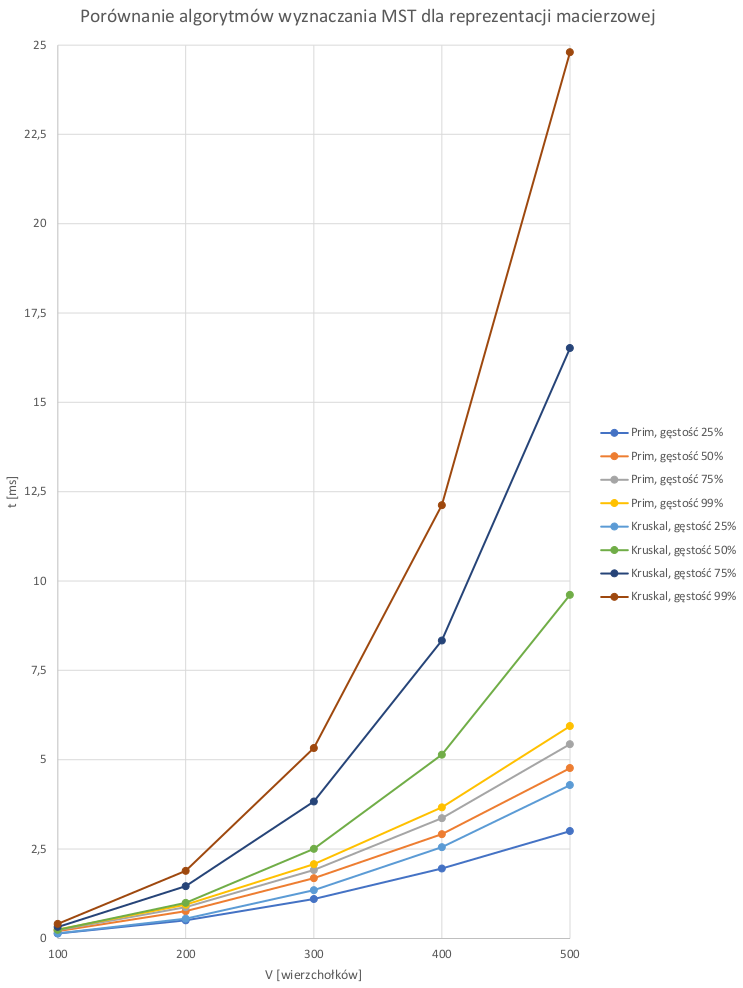
\includegraphics[width=14cm]{fig5.png}
	\label{fig.wykres-macierz-mst}
\end{figure}

\begin{figure}[H]
	\centering
	\caption{\centering Wykres porównujący czasy wykonywania algorytmów wyznaczania MST dla reprezentacji listowej.}
	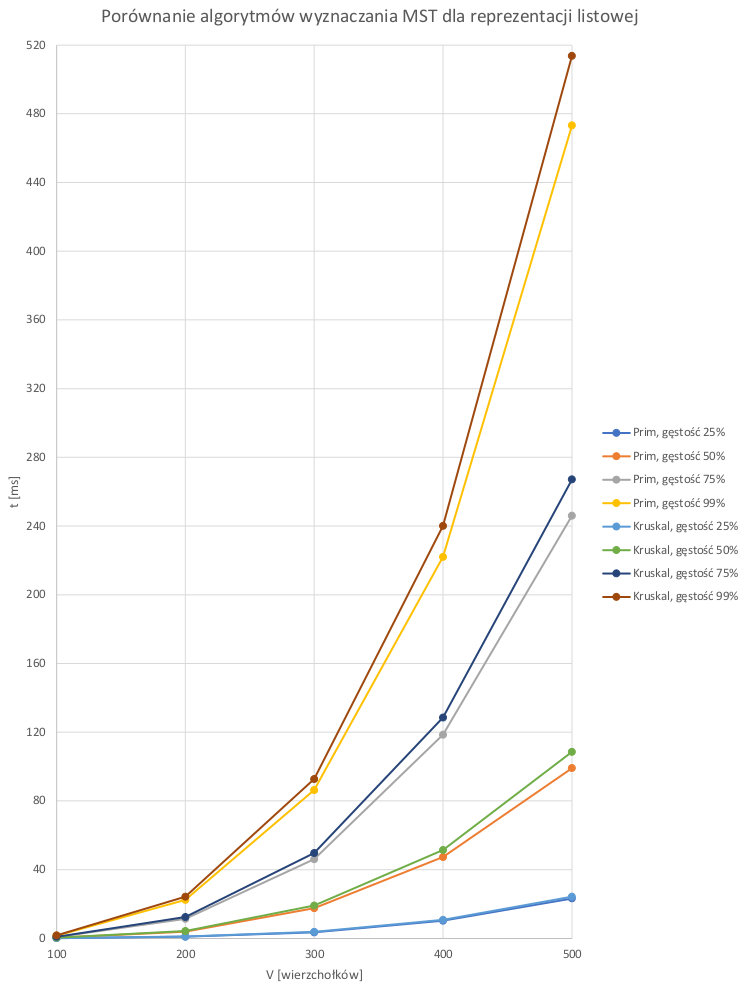
\includegraphics[width=14cm]{fig6.png}
	\label{fig.wykres-lista-mst}
\end{figure}

\subsection{Analiza wyników pomiarów:}

\subsubsection{Algorytm Prima - reprezentacja macierzowa:}
Przyglądając się wartości parametru $c$ oraz jego względnemu odchyleniu standardowemu można zauważyć, że złożoność algorytmu Prima dla reprezentacji macierzowej nie jest do końca zgodna z teoretyczną złożonością $O(E \cdot \log V)$. Wynika to prawdopodobnie z opisywanych wcześniej decyzji dotyczącej rozmiaru kopca. W teoretycznej implementacji może on zwierać $V$ elementów, w mierzonej może przechowywać nawet do $E$ elementów. Można zaryzykować zatem stwierdzenie, że rzeczywista złożoność czasowa algorytmu Prima jest bliższa $O(E \cdot \log E)$ niż teoretycznie postulowanej $O(E \cdot \log V)$.\\

\subsubsection{Algorytm Kruskala - reprezentacja macierzowa:}
W wypadku algorytmu Kruskala dla reprezentacji macierzowej rozbieżności z teoretyczną zależnością są znacznie bardziej zauważalne. Przyglądając się wykresowi porównującemu czas wykonywania się algorytmów wyznaczających MST, można zauważyć, że w przypadku algorytmu Kruskala wzrost wartości jest znacznie szybszy niż w wypadku algorytmu Prima. Jest on znacznie bardziej zbliżony do wzrostu funkcji klasy wielomianowej. Powodem takich odchyleń od zależności teoretycznej jest najprawdopodobniej użycie wewnątrz algorytmu metody zwracającej listę krawędzi grafu (rys. \ref{fig.kruskal-macierz-wyjasnienie-1}). Po przeanalizowaniu jej kodu (rys. \ref{fig.kruskal-macierz-wyjasnienie-2}) można zauważyć, że ma ona złożoność $O(V \cdot E)$, a dla grafu nieskierowanego $O(V^3)$.
\begin{figure}[H]
	\centering
	\caption{\centering Wydruk kodu przedstawiający użycie metody zwracającej listę krawędzi wewnątrz metody implementującej algorytm Kruskala dla grafu w reprezentacji macierzowej.}
	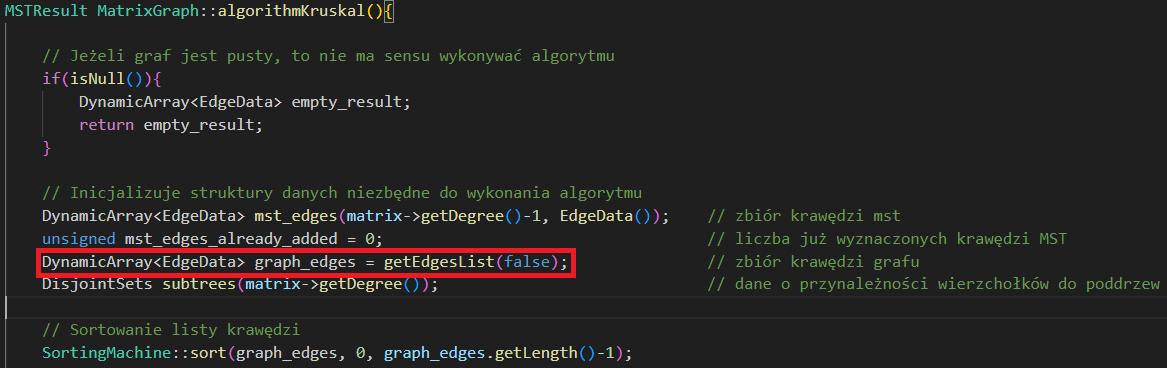
\includegraphics[width=14cm]{fig7.png}
	\label{fig.kruskal-macierz-wyjasnienie-1}
\end{figure}

\begin{figure}[H]
	\centering
	\caption{\centering Wydruk kodu metody zwracającej listę krawędzi dla reprezentacji macierzowej.}
	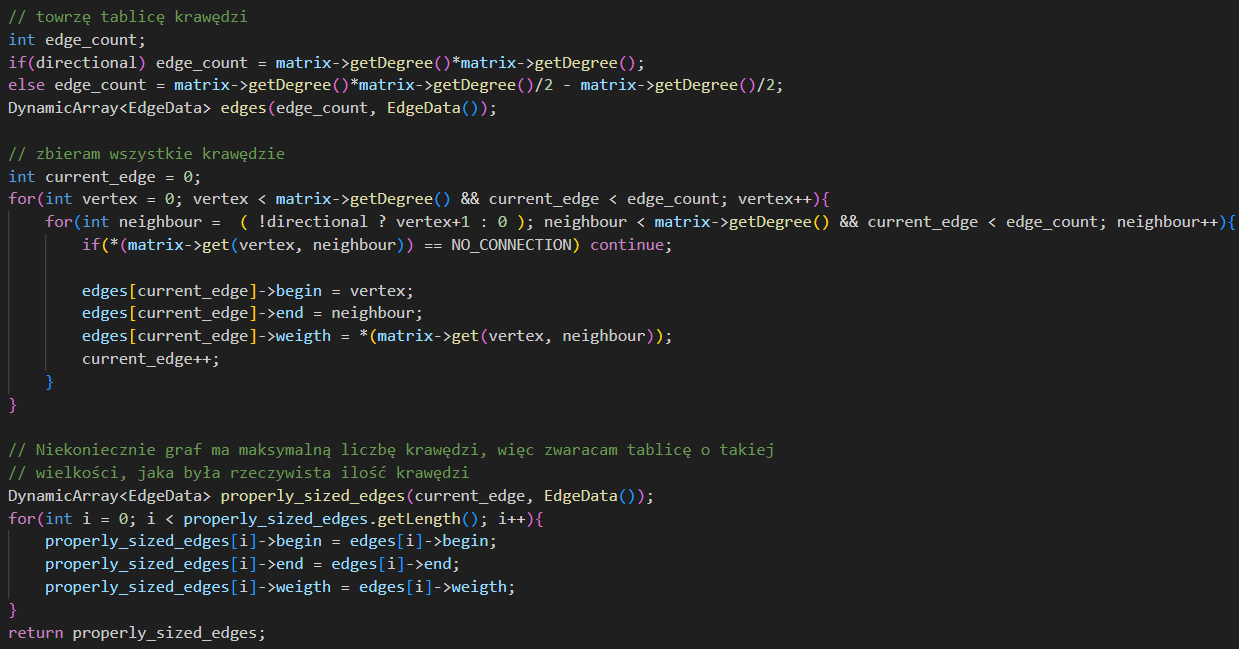
\includegraphics[width=14cm]{fig8.png}
	\label{fig.kruskal-macierz-wyjasnienie-2}
\end{figure}

\subsubsection{Reprezentacje listowe:}
Dla obu rozważanych algorytmów działających na grafach w reprezentacji listowej można zauważyć kompletny brak zgodności z teorią. Także na wykresach widocznym jest fakt, że obie zmierzone zależności rosną w bardzo szybkim tempie. Ów wzrost jest ponadto raczej bliższy charakterystyce wielomianowej niż teoretycznej $(E \cdot \log V)$. Jest to spowodowane złożonością operacji pobierania elementu z listy, która wynosi $O(V)$.\\

\noindent
Ponadto w wypadku algorytmu Kruskala ponownie kosztownym okazało się wytworzenie samej listy krawędzi. Ta operacja także wymagała wielokrotnego dostępu do elementów listy.

%-------------------------------------------------------
%	WYZNACZANIE MINIMALNEGO DRZEWA SPINAJĄCEGO
\section{Wyznaczanie najkrótszej ścieżki:}

\subsection{Algorytm Dijkstry:}

\subsubsection{Opis teoretyczny:}
Algorytm Dijkstry jest algorytmem grafowym, pozwalającym na wyszukiwanie najkrótszych ścieżek z wybranego wierzchołka startowego do wszystkich innych wierzchołków. Zakłada przy tym, że graf, na którym wykonywany jest algorytm jest grafem spójny, o krawędziach skierowanych, których wagi są nieujemne.\\

\noindent
Pierwszym krokiem algorytmu jest wybranie wierzchołka startowego. Następnie, w kolejnych iteracjach odwiedzani są coraz bardziej odległe od tegoż wierzchołki grafu. Kolejność odwiedzin definiowana jest przez łączną odległość od wierzchołka startowego. Pierwsze w kolejności są wierzchołki grafu o minimalnej odległości od punktu startu. Istotną częścią algorytmu Dijkstry jest proces tzw. relaksacji. Polega on na ciągłym wyszukiwaniu coraz to lepszych (krótszych) dróg do jeszcze nieodwiedzonych wierzchołków w każdej iteracji algorytmu.\\

\noindent
Książkowa implementacja algorytmu zakłada użycie kolejki priorytetowej (kopca minimalnego), przechowującej informacje o ścieżkach prowadzących do poszczególnych wierzchołków. Pozwala to na szybki dostęp do tego wierzchołka grafu, którego odległość od punktu startowego będzie najmniejsza. Taki dostęp będzie mieć złożoność jednostkową $O(1)$. Dodawanie lub aktualizacja informacji o wierzchołku do wspomnianej kolejki będzie miała złożoność $O(\log V)$. W celu znalezienia najlepszych ścieżek (relaksacja) musimy rozważyć wszystkie krawędzie grafu, zatem wspominane operacje należy powtórzyć w najgorszym wypadku $E$ razy. Zatem ostateczna złożoność algorytmu wynosi $O (E \cdot \log V)$.

\subsubsection{Zastosowana implementacja:}
Przy implementacji algorytmu Dijkstry wykorzystano kolejkę priorytetową. Była ona de facto zmodyfikowanym kopcem, stworzonym na potrzeby poprzedniego zadania projektowego. Zamiast liczb całkowitych ze znakiem przechowywał on strukturę o polach: indeks wierzchołka, sąsiad z przypisanej krawędzi, waga przypisanej krawędzi. W celu zoptymalizowania operacji dodawania i usuwania elementów pozbyto się przymusu każdorazowej relokacji kopca, występującego przy tychże działaniach. Dokonano tego poprzez zwirtualizowanie tychże operacji. Rzeczywisty rozmiar tablicy, na której bazował kopiec pozostawał stały. Zmniejszany bądź zwiększany był jedynie jej obszar uznawany w danym momencie za właściwy kopiec.\\

\noindent
W projekcie zrezygnowano także z tradycyjnej relaksacji elementów kolejki. Zamiast tego do kopca były za każdym razem dodawane nowe elementy (o ile opisywany przez nie wierzchołek nie był jeszcze odwiedzony). Jeżeli okazałyby się one wagowo korzystniejsze od poprzednich, to prawa rządzące kolejką sprawiały, że były one pobierane wcześniej od swoich gorszych pod tych względem "kopii" (elementów opisujących ten sam wierzchołek, ale z przypisaną inną wagą). Po przy pierwszym pobraniu z kolejki wierzchołek oznaczany był jako odwiedzony, co blokowało możliwość odwiedzenia go ponownie, przy pobraniu jego "kopii" z kopca. Zdecydowano się na takie rozwiązanie ze względu na fakt, że zwykła relaksacja wymagałaby wyszukania w kopcu elementu odpowiadającego danemu wierzchołkowi i następnie jego zmodyfikowanie. Wyszukiwanie elementu w takim wypadku ma złożoność klasy $O(V)$. Znacznie spowolniłoby to cały algorytm, dlatego zdecydowano się na pominięcie tegoż kroku.

\subsection{Algorytm Bellmana-Forda:}

\subsubsection{Opis teoretyczny:}
Algorytm Bellmana-Forda jest algorytmem grafowym, pozwalającym na wyszukiwanie najkrótszych ścieżek z wybranego wierzchołka startowego do wszystkich innych wierzchołków. Zakłada przy tym, że gra, na którym wykonywany jest algorytm jest grafem spójnym, o krawędziach skierowanych. W przeciwieństwie do algorytmu Dijkstry dopuszczalne są ujemne wagi krawędzi.\\

\noindent
Pierwszym krokiem algorytmu jest wybranie wierzchołka startowego i ustalenia odległości innych wierzchołków od tegoż na nieskończoność. Samemu wierzchołkowi startowemu przypisuje się odległość równą zero. Następnie wykonuje się $|V|-1$ relaksacji. Odbywają się one poprzez przeszukanie listy krawędzi w poszukiwaniu jak coraz to krótszych ścieżek do każdego z wierzchołków. Po tym wykonywane jest sprawdzenie, czy graf zawiera cykl ujemny. Jeżeli w grafie taki wystąpi, to algorytm nie zwróci poprawnego wyniku.\\

\noindent
W implementacji zgodnej z teorią musimy przeiterować się $V-1$ razy przez $E$-elemntową listę krawędzi grafu. Dodatkowo w celu sprawdzenia wystąpienia cyklu ujemnego najczęściej wykonuje się dodatkową iterację przez listę krawędzi. W związku z tym złożoność tego algorytmu wynosi $O(E \cdot V)$, co dla grafu skierowanego oznacza de facto złożoność czasową $O(V^3)$.

\subsubsection{Zastosowana implementacja:}
Implementacja w projekcie była w dużym stopniu zgodna z tą teoretyczną. Wprowadzono do niej jedynie drobne poprawki, pozwalające na częściowe skrócenie czasu wykonywania się algorytmu. Pierwszą z nich jest użycie flagi logicznej informującej, czy w danej iteracji nastąpiła jakakolwiek relaksacja. Znalezienie się jej w stanie niskim, oznacza, że algorytm można zakończyć przedwcześnie (gdyż uzyskano już najlepsze możliwe ścieżki). Drugą zmianą jest wprowadzenie dodatkowej $V$-tej iteracji w głównej pętli algorytmu. Jej rozpoczęcie pozwalało na łatwe i przejrzyste uzyskanie informacji o istnieniu cyklu ujemnego w grafie (bo ścieżki nieustannie poprawiały). 

\subsection{Wyniki pomiarów:}

\begin{table}[H]
	\centering
	\caption{\centering Wyniki pomiarów dla algorytmu Dijkstry wykonywanego na grafie w reprezentacji macierzowej o gęstości 25\%.}
	\begin{tabular}{|c|c|c|c|c|c|}
		\hline
		\rowcolor[HTML]{C0C0C0} 
		$R$                       & $d$                    & $V$ & $t$    & $c$                & $\sigma$               \\ \hline
		&                        & 100 & 0,31ms & 1,9$\cdot 10^{-5}$ &                        \\ \cline{3-5}
		&                        & 200 & 1,5ms  & 2,0$\cdot 10^{-5}$ &                        \\ \cline{3-5}
		&                        & 300 & 2,8ms  & 1,5$\cdot 10^{-5}$ &                        \\ \cline{3-5}
		&                        & 400 & 5,2ms  & 1,5$\cdot 10^{-5}$ &                        \\ \cline{3-5}
		\multirow{-5}{*}{macierz} & \multirow{-5}{*}{25\%} & 500 & 8,0ms  & 1,4$\cdot 10^{-5}$ & \multirow{-5}{*}{16\%} \\ \hline
	\end{tabular}
\end{table}

\begin{table}[H]
	\centering
	\caption{\centering Wyniki pomiarów dla algorytmu Dijkstry wykonywanego na grafie w reprezentacji macierzowej o gęstości 50\%.}
	\begin{tabular}{|c|c|c|c|c|c|}
		\hline
		\rowcolor[HTML]{C0C0C0} 
		$R$                       & $d$                    & $V$ & $t$    & $c$                & $\sigma$                \\ \hline
		&                        & 100 & 0,49ms & 1,5$\cdot 10^{-5}$ &                         \\ \cline{3-5}
		&                        & 200 & 2,1ms  & 1,4$\cdot 10^{-5}$ &                         \\ \cline{3-5}
		&                        & 300 & 5,2ms  & 1,4$\cdot 10^{-5}$ &                         \\ \cline{3-5}
		&                        & 400 & 9,5ms  & 1,4$\cdot 10^{-5}$ &                         \\ \cline{3-5}
		\multirow{-5}{*}{macierz} & \multirow{-5}{*}{50\%} & 500 & 15ms   & 1,3$\cdot 10^{-5}$ & \multirow{-5}{*}{3,4\%} \\ \hline
	\end{tabular}
\end{table}

\begin{table}[H]
	\centering
	\caption{\centering Wyniki pomiarów dla algorytmu Dijkstry wykonywanego na grafie w reprezentacji macierzowej o gęstości 75\%.}
	\begin{tabular}{|c|c|c|c|c|c|}
		\hline
		\rowcolor[HTML]{C0C0C0} 
		$R$                       & $d$                    & $V$ & $t$    & $c$                & $\sigma$                \\ \hline
		&                        & 100 & 0,68ms & 1,4$\cdot 10^{-5}$ &                         \\ \cline{3-5}
		&                        & 200 & 3,0ms  & 1,3$\cdot 10^{-5}$ &                         \\ \cline{3-5}
		&                        & 300 & 7,5ms  & 1,4$\cdot 10^{-5}$ &                         \\ \cline{3-5}
		&                        & 400 & 13ms   & 1,3$\cdot 10^{-5}$ &                         \\ \cline{3-5}
		\multirow{-5}{*}{macierz} & \multirow{-5}{*}{75\%} & 500 & 21ms   & 1,3$\cdot 10^{-5}$ & \multirow{-5}{*}{3,4\%} \\ \hline
	\end{tabular}
\end{table}

\begin{table}[H]
	\centering
	\caption{\centering Wyniki pomiarów dla algorytmu Dijkstry wykonywanego na grafie w reprezentacji macierzowej o gęstości 99\%.}
	\begin{tabular}{|c|c|c|c|c|c|}
		\hline
		\rowcolor[HTML]{C0C0C0} 
		$R$                       & $d$                    & $V$ & $t$    & $c$                & $\sigma$                \\ \hline
		&                        & 100 & 0,87ms & 1,3$\cdot 10^{-5}$ &                         \\ \cline{3-5}
		&                        & 200 & 3,8ms  & 1,3$\cdot 10^{-5}$ &                         \\ \cline{3-5}
		&                        & 300 & 9,3ms  & 1,3$\cdot 10^{-5}$ &                         \\ \cline{3-5}
		&                        & 400 & 17ms   & 1,2$\cdot 10^{-5}$ &                         \\ \cline{3-5}
		\multirow{-5}{*}{macierz} & \multirow{-5}{*}{99\%} & 500 & 27ms   & 1,2$\cdot 10^{-5}$ & \multirow{-5}{*}{3,1\%} \\ \hline
	\end{tabular}
\end{table}

\begin{table}[H]
	\centering
	\caption{\centering Wyniki pomiarów dla algorytmu Bellmana-Forda wykonywanego na grafie w reprezentacji macierzowej o gęstości 25\%.}
	\begin{tabular}{|c|c|c|c|c|c|}
		\hline
		\rowcolor[HTML]{C0C0C0} 
		$R$                       & $d$                    & $V$ & $t$   & $c$                & $\sigma$                \\ \hline
		&                        & 100 & 2,4ms & 9,4$\cdot 10^{-6}$ &                         \\ \cline{3-5}
		&                        & 200 & 18ms  & 9,2$\cdot 10^{-6}$ &                         \\ \cline{3-5}
		&                        & 300 & 62ms  & 9,2$\cdot 10^{-6}$ &                         \\ \cline{3-5}
		&                        & 400 & 150ms & 9,2$\cdot 10^{-6}$ &                         \\ \cline{3-5}
		\multirow{-5}{*}{macierz} & \multirow{-5}{*}{25\%} & 500 & 290ms & 9,1$\cdot 10^{-6}$ & \multirow{-5}{*}{1,2\%} \\ \hline
	\end{tabular}
\end{table}

\begin{table}[H]
	\centering
	\caption{\centering Wyniki pomiarów dla algorytmu Bellmana-Forda wykonywanego na grafie w reprezentacji macierzowej o gęstości 50\%.}
	\begin{tabular}{|c|c|c|l|c|c|}
		\hline
		\rowcolor[HTML]{C0C0C0} 
		$R$                       & $d$                    & $V$ & \multicolumn{1}{c|}{\cellcolor[HTML]{C0C0C0}$t$} & $c$                & $\sigma$                 \\ \hline
		&                        & 100 & 4,6ms                                            & 9,3$\cdot 10^{-6}$ &                          \\ \cline{3-5}
		&                        & 200 & 37ms                                             & 9,2$\cdot 10^{-6}$ &                          \\ \cline{3-5}
		&                        & 300 & 120ms                                            & 9,2$\cdot 10^{-6}$ &                          \\ \cline{3-5}
		&                        & 400 & 290ms                                            & 9,2$\cdot 10^{-6}$ &                          \\ \cline{3-5}
		\multirow{-5}{*}{macierz} & \multirow{-5}{*}{50\%} & 500 & 570ms                                            & 9,1$\cdot 10^{-6}$ & \multirow{-5}{*}{0,60\%} \\ \hline
	\end{tabular}
\end{table}

\begin{table}[H]
	\centering
	\caption{\centering Wyniki pomiarów dla algorytmu Bellmana-Forda wykonywanego na grafie w reprezentacji macierzowej o gęstości 75\%.}
	\begin{tabular}{|c|c|c|c|c|c|}
		\hline
		\rowcolor[HTML]{C0C0C0} 
		$R$                       & $d$                    & $V$ & $t$   & $c$                & $\sigma$                 \\ \hline
		&                        & 100 & 7,0ms & 9,3$\cdot 10^{-6}$ &                          \\ \cline{3-5}
		&                        & 200 & 56ms  & 9,3$\cdot 10^{-6}$ &                          \\ \cline{3-5}
		&                        & 300 & 190ms & 9,3$\cdot 10^{-6}$ &                          \\ \cline{3-5}
		&                        & 400 & 440ms & 9,2$\cdot 10^{-6}$ &                          \\ \cline{3-5}
		\multirow{-5}{*}{macierz} & \multirow{-5}{*}{75\%} & 500 & 860ms & 9,2$\cdot 10^{-6}$ & \multirow{-5}{*}{0,65\%} \\ \hline
	\end{tabular}
\end{table}

\begin{table}[H]
	\centering
	\caption{\centering Wyniki pomiarów dla algorytmu Bellmana-Forda wykonywanego na grafie w reprezentacji macierzowej o gęstości 99\%.}
	\begin{tabular}{|c|c|c|c|c|c|}
		\hline
		\rowcolor[HTML]{C0C0C0} 
		$R$                       & $d$                    & $V$ & \multicolumn{1}{c|}{\cellcolor[HTML]{C0C0C0}$t$} & $c$                & $\sigma$                 \\ \hline
		&                        & 100 & 9,6ms                                            & 9,3$\cdot 10^{-6}$ &                          \\ \cline{3-5}
		&                        & 200 & 74ms                                             & 9,3$\cdot 10^{-6}$ &                          \\ \cline{3-5}
		&                        & 300 & 250ms                                            & 9,3$\cdot 10^{-6}$ &                          \\ \cline{3-5}
		&                        & 400 & 590ms                                            & 9,3$\cdot 10^{-6}$ &                          \\ \cline{3-5}
		\multirow{-5}{*}{macierz} & \multirow{-5}{*}{99\%} & 500 & 1,1s                                             & 9,2$\cdot 10^{-6}$ & \multirow{-5}{*}{0,49\%} \\ \hline
	\end{tabular}
\end{table}

\begin{table}[H]
	\centering
	\caption{\centering Wyniki pomiarów dla algorytmu Dijkstry wykonywanego na grafie w reprezentacji listowej o gęstości 25\%.}
	\begin{tabular}{|c|c|c|c|c|c|}
		\hline
		\rowcolor[HTML]{C0C0C0} 
		$R$                       & $d$                    & $V$ & $t$    & $c$                & $\sigma$               \\ \hline
		&                        & 100 & 0,31ms & 1,9$\cdot 10^{-5}$ &                        \\ \cline{3-5}
		&                        & 200 & 1,5ms  & 2,0$\cdot 10^{-5}$ &                        \\ \cline{3-5}
		&                        & 300 & 5,1ms  & 2,8$\cdot 10^{-5}$ &                        \\ \cline{3-5}
		&                        & 400 & 13ms   & 3,8$\cdot 10^{-5}$ &                        \\ \cline{3-5}
		\multirow{-5}{*}{lista} & \multirow{-5}{*}{25\%} & 500 & 28ms   & 5,0$\cdot 10^{-5}$ & \multirow{-5}{*}{43\%} \\ \hline
	\end{tabular}
\end{table}

\begin{table}[H]
	\centering
	\caption{\centering Wyniki pomiarów dla algorytmu Dijkstry wykonywanego na grafie w reprezentacji listowej o gęstości 50\%.}
	\begin{tabular}{|c|c|c|c|c|c|}
		\hline
		\rowcolor[HTML]{C0C0C0} 
		$R$                       & $d$                    & $V$ & $t$    & $c$                & $\sigma$               \\ \hline
		&                        & 100 & 0,70ms & 2,1$\cdot 10^{-5}$ &                        \\ \cline{3-5}
		&                        & 200 & 4,2ms  & 2,7$\cdot 10^{-5}$ &                        \\ \cline{3-5}
		&                        & 300 & 13ms   & 3,5$\cdot 10^{-5}$ &                        \\ \cline{3-5}
		&                        & 400 & 29ms   & 4,2$\cdot 10^{-5}$ &                        \\ \cline{3-5}
		\multirow{-5}{*}{lista} & \multirow{-5}{*}{50\%} & 500 & 56ms   & 5,0$\cdot 10^{-5}$ & \multirow{-5}{*}{32\%} \\ \hline
	\end{tabular}
\end{table}

\begin{table}[H]
	\centering
	\caption{\centering Wyniki pomiarów dla algorytmu Dijkstry wykonywanego na grafie w reprezentacji listowej o gęstości 75\%.}
	\begin{tabular}{|c|c|c|c|c|c|}
		\hline
		\rowcolor[HTML]{C0C0C0} 
		$R$                     & $d$                    & $V$ & \multicolumn{1}{c|}{\cellcolor[HTML]{C0C0C0}$t$} & $c$                & $\sigma$               \\ \hline
		&                        & 100 & 1,3ms                                            & 2,5$\cdot 10^{-5}$ &                        \\ \cline{3-5}
		&                        & 200 & 8,5ms                                            & 3,7$\cdot 10^{-5}$ &                        \\ \cline{3-5}
		&                        & 300 & 27ms                                             & 4,9$\cdot 10^{-5}$ &                        \\ \cline{3-5}
		&                        & 400 & 62ms                                             & 5,9$\cdot 10^{-5}$ &                        \\ \cline{3-5}
		\multirow{-5}{*}{lista} & \multirow{-5}{*}{75\%} & 500 & 120ms                                            & 7,0$\cdot 10^{-5}$ & \multirow{-5}{*}{37\%} \\ \hline
	\end{tabular}
\end{table}

\begin{table}[H]
	\centering
	\caption{\centering Wyniki pomiarów dla algorytmu Dijkstry wykonywanego na grafie w reprezentacji listowej o gęstości 99\%.}
	\begin{tabular}{|c|c|c|c|c|c|}
		\hline
		\rowcolor[HTML]{C0C0C0} 
		$R$                     & $d$                    & $V$ & \multicolumn{1}{c|}{\cellcolor[HTML]{C0C0C0}$t$} & $c$                & $\sigma$               \\ \hline
		&                        & 100 & 2,0ms                                            & 3,0$\cdot 10^{-5}$ &                        \\ \cline{3-5}
		&                        & 200 & 14ms                                             & 4,6$\cdot 10^{-5}$ &                        \\ \cline{3-5}
		&                        & 300 & 45ms                                             & 6,1$\cdot 10^{-5}$ &                        \\ \cline{3-5}
		&                        & 400 & 100ms                                            & 7,6$\cdot 10^{-5}$ &                        \\ \cline{3-5}
		\multirow{-5}{*}{lista} & \multirow{-5}{*}{99\%} & 500 & 200ms                                            & 9,0$\cdot 10^{-5}$ & \multirow{-5}{*}{39\%} \\ \hline
	\end{tabular}
\end{table}

\begin{table}[H]
	\centering
	\caption{\centering Wyniki pomiarów dla algorytmu Bellmana-Forda wykonywanego na grafie w reprezentacji listowej o gęstości 25\%.}
	\begin{tabular}{|c|c|c|c|c|c|}
		\hline
		\rowcolor[HTML]{C0C0C0} 
		$R$                     & $d$                    & $V$ & \multicolumn{1}{c|}{\cellcolor[HTML]{C0C0C0}$t$} & $c$                & $\sigma$                \\ \hline
		&                        & 100 & 2,2ms                                            & 8,9$\cdot 10^{-6}$ &                         \\ \cline{3-5}
		&                        & 200 & 18ms                                             & 9,0$\cdot 10^{-6}$ &                         \\ \cline{3-5}
		&                        & 300 & 61ms                                             & 9,1$\cdot 10^{-6}$ &                         \\ \cline{3-5}
		&                        & 400 & 150ms                                            & 9,2$\cdot 10^{-6}$ &                         \\ \cline{3-5}
		\multirow{-5}{*}{lista} & \multirow{-5}{*}{25\%} & 500 & 290ms                                            & 9,3$\cdot 10^{-6}$ & \multirow{-5}{*}{1,7\%} \\ \hline
	\end{tabular}
\end{table}

\begin{table}[H]
	\centering
	\caption{\centering Wyniki pomiarów dla algorytmu Bellmana-Forda wykonywanego na grafie w reprezentacji listowej o gęstości 50\%.}
	\begin{tabular}{|c|c|c|c|c|c|}
		\hline
		\rowcolor[HTML]{C0C0C0} 
		$R$                     & $d$                    & $V$ & \multicolumn{1}{c|}{\cellcolor[HTML]{C0C0C0}$t$} & $c$                & $\sigma$                 \\ \hline
		&                        & 100 & 4,6ms                                            & 9,2$\cdot 10^{-6}$ &                          \\ \cline{3-5}
		&                        & 200 & 37ms                                             & 9,3$\cdot 10^{-6}$ &                          \\ \cline{3-5}
		&                        & 300 & 130ms                                            & 9,3$\cdot 10^{-6}$ &                          \\ \cline{3-5}
		&                        & 400 & 300ms                                            & 9,3$\cdot 10^{-6}$ &                          \\ \cline{3-5}
		\multirow{-5}{*}{lista} & \multirow{-5}{*}{50\%} & 500 & 580ms                                            & 9,3$\cdot 10^{-6}$ & \multirow{-5}{*}{0,51\%} \\ \hline
	\end{tabular}
\end{table}

\begin{table}[H]
	\centering
	\caption{\centering Wyniki pomiarów dla algorytmu Bellmana-Forda wykonywanego na grafie w reprezentacji listowej o gęstości 75\%.}
	\begin{tabular}{|c|c|c|c|c|c|}
		\hline
		\rowcolor[HTML]{C0C0C0} 
		$R$                     & $d$                    & $V$ & $t$   & $c$                & $\sigma$                 \\ \hline
		&                        & 100 & 7,2ms & 9,6$\cdot 10^{-6}$ &                          \\ \cline{3-5}
		&                        & 200 & 58ms  & 9,7$\cdot 10^{-6}$ &                          \\ \cline{3-5}
		&                        & 300 & 200ms & 9,7$\cdot 10^{-6}$ &                          \\ \cline{3-5}
		&                        & 400 & 470ms & 9,7$\cdot 10^{-6}$ &                          \\ \cline{3-5}
		\multirow{-5}{*}{lista} & \multirow{-5}{*}{75\%} & 500 & 910ms & 9,8$\cdot 10^{-6}$ & \multirow{-5}{*}{0,72\%} \\ \hline
	\end{tabular}
\end{table}

\begin{table}[H]
	\centering
	\caption{\centering Wyniki pomiarów dla algorytmu Bellmana-Forda wykonywanego na grafie w reprezentacji listowej o gęstości 99\%.}
	\begin{tabular}{|c|c|c|c|c|c|}
		\hline
		\rowcolor[HTML]{C0C0C0} 
		$R$                     & $d$                    & $V$ & $t$   & $c$                & $\sigma$                 \\ \hline
		&                        & 100 & 9,6ms & 1,0$\cdot 10^{-5}$ &                          \\ \cline{3-5}
		&                        & 200 & 80ms  & 1,0$\cdot 10^{-5}$ &                          \\ \cline{3-5}
		&                        & 300 & 270ms & 1,0$\cdot 10^{-5}$ &                          \\ \cline{3-5}
		&                        & 400 & 640ms & 1,0$\cdot 10^{-5}$ &                          \\ \cline{3-5}
		\multirow{-5}{*}{lista} & \multirow{-5}{*}{99\%} & 500 & 1,3s  & 1,0$\cdot 10^{-5}$ & \multirow{-5}{*}{0,81\%} \\ \hline
	\end{tabular}
\end{table}

\begin{figure}[H]
	\centering
	\caption{\centering Wykres porównujący czasy wykonywania algorytmów wyszukiwania najkrótszej ścieżki dla reprezentacji macierzowej.}
	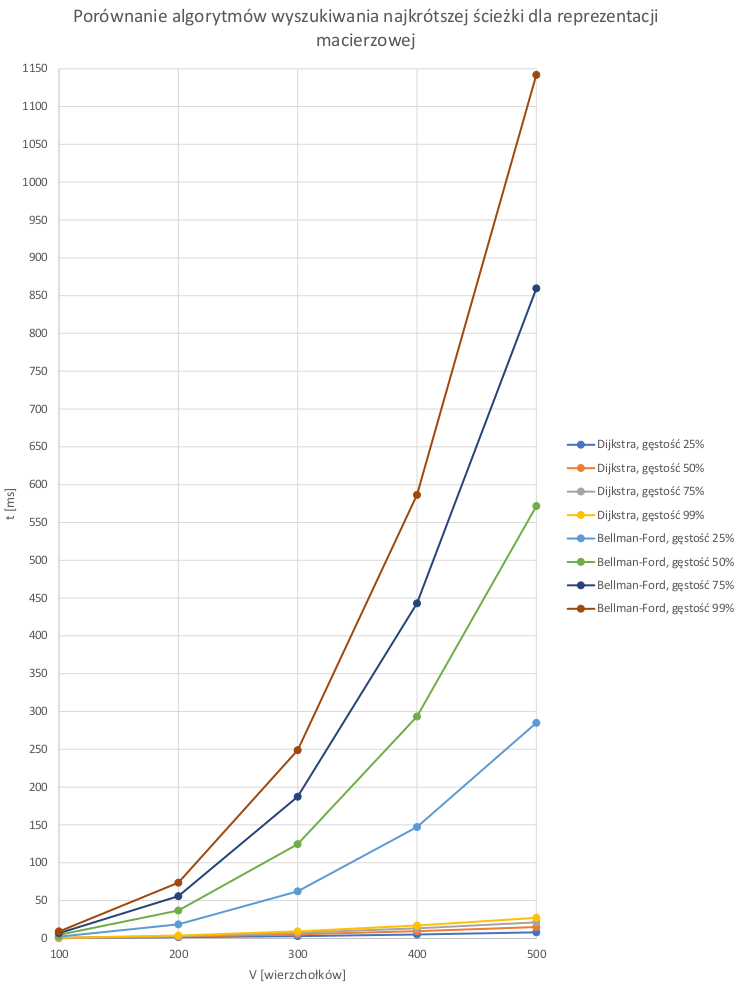
\includegraphics[width=14cm]{fig4.png}
	\label{fig.wykres-macierz-shortpath}
\end{figure}

\begin{figure}[H]
	\centering
	\caption{\centering Wykres porównujący czasy wykonywania algorytmów wyszukiwania najkrótszej ścieżki dla reprezentacji listowej.}
	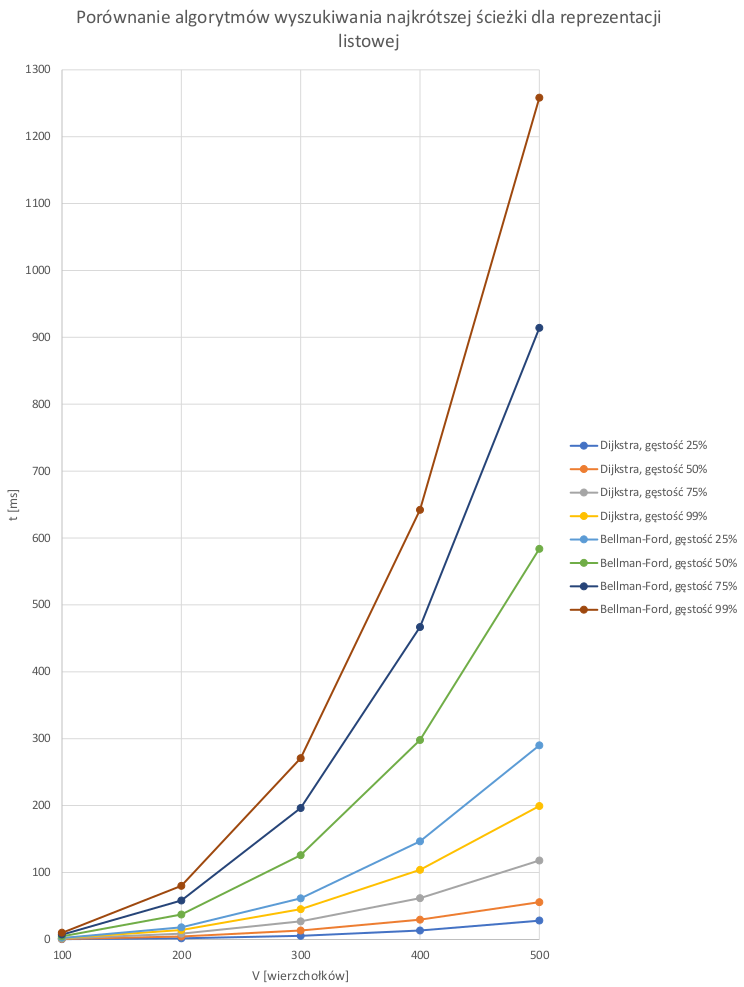
\includegraphics[width=14cm]{fig3.png}
	\label{fig.wykres-lista-shortpath}
\end{figure}

\subsection{Analiza wyników pomiarów:}

\subsubsection{Algorytm Bellmana-Forda:}
W wypadku algorytmu Bellmana-Forda wyniki pomiarów wydają się być dosyć dobrze zbliżone do teoretycznej złożoności czasowej $O(V^3)$. Warto jednak zaznaczyć, że wypadku obu reprezentacji algorytm Bellmana-Forda okazał być się znacznie bardziej czasowo wymagający od algorytmu Dijkstry.

\subsubsection{Algorytm Dijkstry:}
Dla grafu w reprezentacji macierzowej uzyskane wyniki zdają się być wystarczająco dobrze zbliżone do teoretycznej złożoności czasowej $O(E \cdot \log V)$. \\

\noindent
Co do reprezentacji listowej, to podobnie jak w wypadku algorytmów Prima oraz Kruskala, wystąpiły spore odchylenia od złożoności $O(E \cdot \log V)$. Ponownie winowajcą była złożoność operacji dostępu do elementu wewnątrz listy. Pomimo tego znacznego spowolnienia algorytm Dijkstry wciąż okazał się szybszy od algorytmu Bellmana-Forda.

%-------------------------------------------------------
%	WNIOSKI
\section{Wnioski:}
Złożoność obliczeniowa dostępu do elementu listy, sprawia, że praktycznie wszystkie algorytmy grafowe dla reprezentacji listowej są znacznie mniej efektywne niż ich odpowiedniki dla reprezentacji macierzowej. W wypadku napisanego projektu większość operacji dostępu do elementów listy odbywało się w ramach iterowania się po jej wszystkich elementach. Stąd można wywnioskować implementacja obiektów-iterwatorów dla tychże list, podobnych do tych obecnych w standardowej bibliotece STL, sprawiłaby, że reprezentacja listowa stałaby się znacznie bardziej konkurencyjna względem tej macierzowej.\\

\noindent
Warto także zauważyć, że w wypadku znajdowania najkrótszej ścieżki użycie algorytmu Bellmana-Forda jest uzasadnione wyłącznie w momencie, gdy istnieje możliwość wystąpienia krawędzi o ujemnych wagach. Jeżeli takie wagi w grafie nie występują, to algorytm Dijkstry będzie praktycznie zawsze lepszym wyborem z perspektywy długości czasu wykonywania.\\

\noindent
Bardzo uciążliwym wąskim gardłem, zwłaszcza w algorytmie Kruskala okazała się być sama operacja wyznaczania krawędzi grafu. Najprostszym rozwiązaniem tego problemu byłoby wytworzenie i zapamiętanie zbioru krawędzi już na etapie tworzenia grafu. Jest to jednak z drugiej strony mało efektywne z punktu widzenia używanej pamięci. Nastąpiłaby wówczas tak naprawdę redundancja danych zawartych w bądź to listach sąsiadów, bądź to macierzy sąsiedztwa.

\end{document}